\chapter{外差式φ-OTDR传感与信号解调原理}

\section{引言}

本章建立第三章发射链路与DAS一体化收发模组实验、第四章数字相位解调与系统验证所需的统一物理模型和信号模型。首先从声波引起的光纤形变出发，说明几何效应和光弹效应如何共同调制传播相位；继而讨论瑞利散射、传统OTDR、相位敏感型OTDR（phase-sensitive optical time-domain reflectometry，φ-OTDR）、距离--时间映射、探测方案、性能指标与信号衰落。在此基础上，进一步建立EDFA与SOA工作特性、集成SOA的ECL激光器增益与相位动态、AOM移频、外差平衡探测、数字下变频、差分相位和双偏振接收模型。DAS一体化收发模组的器件布局、封装和接口将在第三章结合系统实现进行讨论。

本章通过SOA载流子—折射率耦合模型描述动态相位和瞬时频率变化的物理途径。第三章将结合电流、脉宽、温度、输入功率、光路延迟、AOM支路和断光对照实验，辨识本文系统中拍频变化的主导机制。

\section{φ-OTDR分布式振动传感原理}

\subsection{外界声波对光纤相位的调制}

声波在介质中表现为随时间和空间传播的压力扰动。标准传感光纤由纤芯、包层和外部涂覆层构成，纤芯与包层的折射率差将光场约束在导模中。传感光缆与被测对象或周围介质发生机械耦合后，声压引起的位移、拉伸和压缩传递至纤芯，使光纤长度、横向尺寸和有效折射率发生变化。对真空波长为$\lambda_0$的单色光，长度为$L$的光纤所产生的单程传播相位为

\begin{equation}
\phi=\beta L=\frac{2\pi}{\lambda_0}n_{\mathrm{eff}}L,
\label{eq:propagation_phase}
\end{equation}

其中，$\beta$为传播常数，$n_{\mathrm{eff}}$为导模有效折射率。在光源频率固定且扰动量较小时，对式\eqref{eq:propagation_phase}作一阶微分可得

\begin{equation}
\delta\phi
=
\frac{2\pi}{\lambda_0}
\left(
n_{\mathrm{eff}}\,\delta L
+L\,\delta n_{\mathrm{eff}}
\right).
\label{eq:phase_total_differential}
\end{equation}

式\eqref{eq:phase_total_differential}中的第一项为几何长度变化产生的相位变化，第二项为应力光学效应产生的折射率变化。若轴向应变为$\varepsilon_z$，则$\delta L=L\varepsilon_z$。对于各向同性石英光纤，在单轴应变和泊松收缩近似下，可将光弹张量的作用归并为等效光弹系数

\begin{equation}
p_e
=
\frac{n_{\mathrm{eff}}^2}{2}
\left[
p_{12}-\nu\left(p_{11}+p_{12}\right)
\right],
\qquad
\frac{\delta n_{\mathrm{eff}}}{n_{\mathrm{eff}}}
\approx-p_e\varepsilon_z,
\label{eq:effective_photoelastic}
\end{equation}

其中，$p_{11}$、$p_{12}$为光弹张量系数，$\nu$为泊松比。对于φ-OTDR中的往返传播以及长度为$L_g$的标距，最终得到的等效差分相位与标距内平均轴向应变近似呈线性关系，即

\begin{equation}
\Delta\phi_\varepsilon(t)
=
\frac{4\pi n_{\mathrm{eff}}L_g}{\lambda_0}
\left(1-p_e\right)\bar{\varepsilon}(t).
\label{eq:acoustic_strain_phase}
\end{equation}

声波、光纤形变、光程和往返相位之间的传递关系如图\ref{fig:chap2_acoustic_phase_chain}所示。实际光缆的护套、铠装层、耦合介质和安装方式会改变声压到纤芯应变的传递函数，因此式\eqref{eq:acoustic_strain_phase}给出的是光纤内部的等效应变--相位关系，而不是脱离封装条件的声压灵敏度。另一方面，单一相位观测量不足以同时独立反演轴向应变与径向应变；只有引入泊松关系、边界条件或多分量观测后，才可进一步区分不同方向的应变分量\cite{posey2000strain,liokumovich2015fundamentals,bhatta2019dynamic}。

\begin{figure}[htbp]
  \centering
  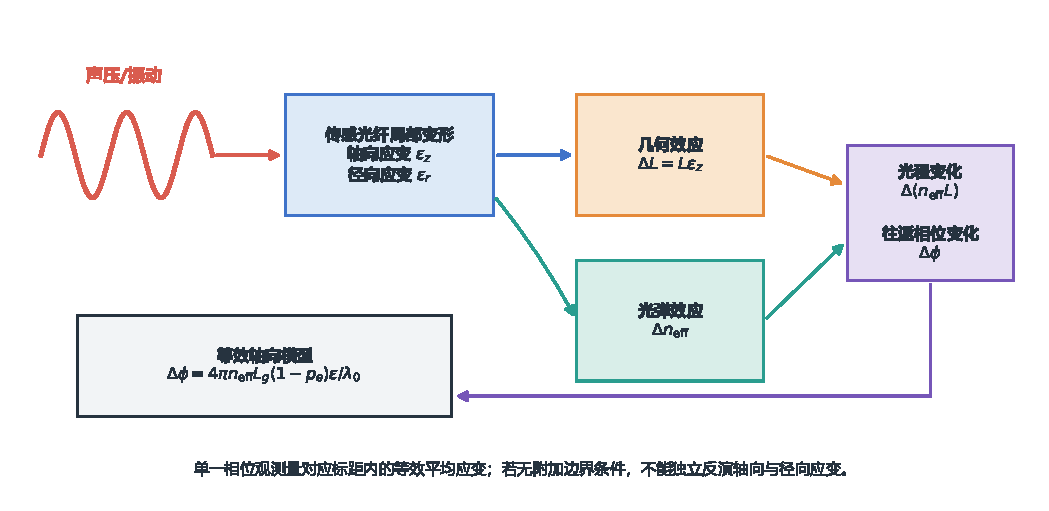
\includegraphics[width=0.96\textwidth]{images/chap2_acoustic_phase_chain.pdf}
  \caption{声波扰动经几何效应与光弹效应转换为光相位变化的过程}
  \label{fig:chap2_acoustic_phase_chain}
\end{figure}

\subsection{相干瑞利后向散射与距离映射}

光纤在制造过程中存在随机微观折射率起伏。当窄线宽光脉冲沿光纤传播时，各微小散射中心产生瑞利后向散射。对于位于距离区间$[z,z+\Delta z]$内的散射中心，接收端复光场可表示为

\begin{equation}
E_{\mathrm R}(z,t)
=
\sum_{k=1}^{M}
a_k
\exp\!\left\{
j\left[
\omega_0 t
-2\beta z_k
+\theta_k
\right]
\right\},
\label{eq:rayleigh_sum}
\end{equation}

其中，$a_k$和$\theta_k$分别为第$k$个等效散射中心的幅度和随机初相，$\omega_0$为光载波角频率，$\beta$为传播常数，$z_k$为散射位置。式\eqref{eq:rayleigh_sum}表明，同一空间分辨单元内的回波由大量随机散射光场相干叠加，其幅度和相位均随空间位置呈现散斑特征\cite{posey2000strain,liokumovich2015fundamentals,he2021review,liu2022advances,liu2025rayleigh_thesis}。

光纤散射按散射前后光频率是否改变可分为弹性散射和非弹性散射。瑞利散射属于弹性散射，其散射光频率与入射光基本相同，因而适合保留并承载入射光的相位信息；拉曼散射和布里渊散射属于非弹性散射，频谱相对入射光发生偏移。φ-OTDR利用耦合回反向导模的瑞利散射分量，而不是把所有方向的散射功率均作为可接收信号。

当一个分辨单元内包含足够多且相互独立的随机散射中心时，合成复场的同相与正交分量可近似视为零均值高斯变量。于是场幅值$A=|E_{\mathrm R}|$近似服从瑞利分布，光强$I=A^2$近似服从指数分布，相位$\Theta$在$[-\pi,\pi)$内近似均匀分布：

\begin{align}
p_A(a)&=\frac{a}{\sigma_R^2}\exp\!\left(-\frac{a^2}{2\sigma_R^2}\right),\quad a\geq0,\label{eq:rayleigh_amplitude_pdf}\\
p_I(i)&=\frac{1}{\bar I}\exp\!\left(-\frac{i}{\bar I}\right),\quad i\geq0,\label{eq:rayleigh_intensity_pdf}\\
p_\Theta(\theta)&=\frac{1}{2\pi},\quad -\pi\leq\theta<\pi.
\label{eq:rayleigh_phase_pdf}
\end{align}

上述统计关系解释了φ-OTDR原始曲线沿距离呈现随机起伏而非平滑衰减的原因。需要特别区分的是，服从瑞利分布的是合成场幅值，而强度服从指数分布；当随机相量近似抵消时，局部幅值可接近零并形成瑞利干涉衰落。

若光纤功率衰减系数为$\alpha(z)$，前向传播功率满足

\begin{equation}
P(z)=P_0\exp\!\left[-\int_0^z\alpha(u)\,\mathrm du\right],
\qquad
\alpha_{\mathrm{dB}}=\frac{10}{\ln 10}\alpha\approx4.343\alpha,
\label{eq:fiber_power_attenuation}
\end{equation}

其中，第二个关系适用于$\alpha$按单位长度的自然对数功率衰减定义且沿程均匀的情形。设$\gamma_b(z)$为单位长度耦合回接收导模的等效后向瑞利功率系数，脉冲在距离维覆盖的单程等效长度为$\ell_p=v_g\tau_p/2$，则忽略器件插损和探测器响应时，传统OTDR在距离$z$附近接收的平均后向散射功率量级可写为

\begin{equation}
P_b(z)
\approx
P_0\,\gamma_b(z)\ell_p
\exp\!\left[-2\int_0^z\alpha(u)\,\mathrm du\right].
\label{eq:otdr_backscatter_power}
\end{equation}

指数项中的系数2来自前向与返回的双程损耗。式\eqref{eq:otdr_backscatter_power}用于说明脉冲能量、后向散射系数和双程衰减的关系；φ-OTDR的瞬时回波还叠加了式\eqref{eq:rayleigh_sum}所描述的相干散斑，不能仅用平均功率曲线代替复场模型。

设光脉冲发出后经过时间$t$被接收，若光纤群折射率为$n_g$，则回波位置近似为

\begin{equation}
z=\frac{ct}{2n_g},
\label{eq:distance_time}
\end{equation}

式中$c$为真空光速，系数2对应光在光纤中的往返传播。数字采样率为$f_s$时，相邻采样点对应的距离间隔为

\begin{equation}
\Delta z_s=\frac{c}{2n_g f_s}.
\label{eq:sample_spacing}
\end{equation}

$\Delta z_s$是距离采样间隔，并不必然等于系统空间分辨率。空间分辨率主要由光脉冲宽度、接收带宽和后续处理共同决定\cite{lu2010distributed,liokumovich2015fundamentals}。

上述脉冲发射、瑞利回波接收和距离映射关系如图\ref{fig:chap2_phi_otdr_principle}所示。光脉冲到达不同位置的散射中心后形成具有不同往返延迟的后向散射光，相干接收与DAQ将连续回波转换为离散采样点，再依据式\eqref{eq:distance_time}和式\eqref{eq:sample_spacing}建立时间索引与空间位置之间的对应关系。

\begin{figure}[htbp]
  \centering
  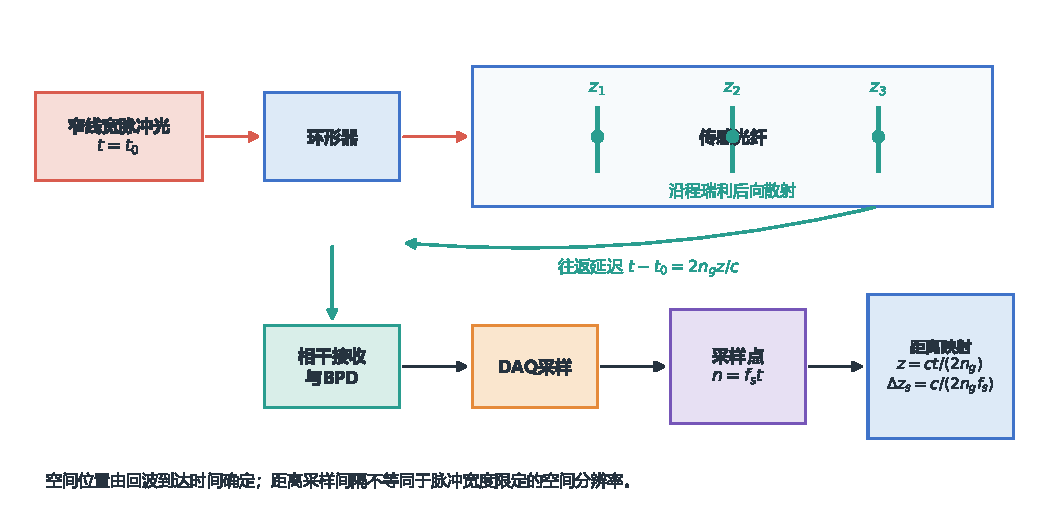
\includegraphics[width=0.96\textwidth]{images/chap2_phi_otdr_principle.pdf}
  \caption{外差式$\varphi$-OTDR瑞利后向散射与距离--时间映射示意图}
  \label{fig:chap2_phi_otdr_principle}
\end{figure}

\subsection{传统OTDR、φ-OTDR及其探测方案}

按扫描变量和定位方式，分布式反射测量可概括为时域反射与频域反射两类。OTDR发射脉冲并依据往返时间定位，适合公里级长距离动态测量；光频域反射计（optical frequency-domain reflectometry，OFDR）通常扫描光频并由拍频或傅里叶变换恢复距离信息，具有较高空间分辨能力，但测距、扫频线性度和动态刷新率受到不同约束。本文研究对象为面向动态振动测量的φ-OTDR，后续模型均采用时域脉冲和慢时间采样框架。

传统OTDR、直接探测型φ-OTDR与本文采用的外差相干型φ-OTDR的信号链如图\ref{fig:chap2_detection_schemes}所示。传统OTDR采用低相干光源时，同一脉冲覆盖范围内的回波主要按功率叠加，所得平滑衰减曲线适合检测光纤长度、损耗、熔接点和断点。φ-OTDR改用窄线宽光源，使局部散射光场发生稳定的相干叠加；外界扰动改变散射相量间的相对相位，进而使回波强度和复相位随慢时间变化\cite{lu2010distributed,masoudi2016review,he2021review}。

\begin{figure}[htbp]
  \centering
  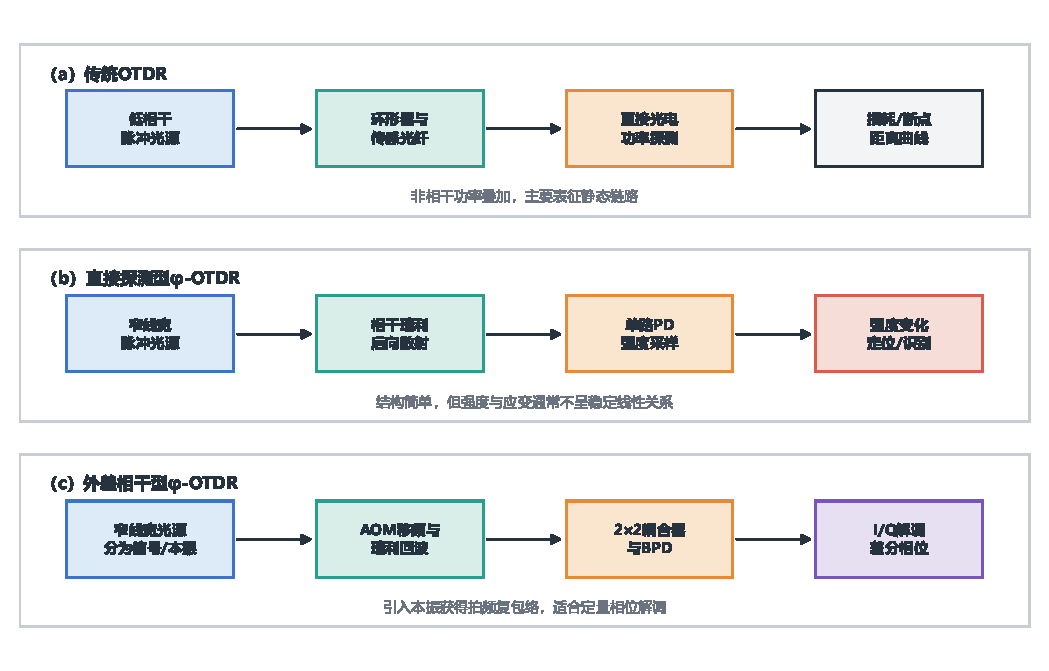
\includegraphics[width=0.96\textwidth]{images/chap2_detection_schemes.pdf}
  \caption{传统OTDR、直接探测型与外差相干型φ-OTDR的信号链对比}
  \label{fig:chap2_detection_schemes}
\end{figure}

根据接收方式，φ-OTDR可进一步分为直接探测、自外差探测和外部本振相干探测。直接探测使用单路光电探测器记录$|E_{\mathrm R}|^2$，结构简单，可利用相邻帧差分或统计量进行扰动定位；然而随机散斑工作点使强度变化与应变一般不保持稳定的线性关系，因此不宜仅凭单点强度定量恢复应变。自外差方案可向光纤注入具有时间间隔和频率差的双脉冲，使两脉冲对应的瑞利回波在探测器上形成拍频，拍频相位反映由脉冲间隔确定的空间区间相位差。外部本振相干探测则将同源连续光作为本振，与返回的瑞利信号光在耦合器和BPD中拍频，通过I/Q解调获得复包络，既利用本振提高弱回波的可检测性，又能在数字域灵活选择差分标距。本文采用最后一种方案，并在本章后半部分给出其完整模型。

\subsection{空间分辨率、测距与采样约束}

若入纤光脉冲持续时间为$\tau_p$，忽略脉冲整形和接收带宽的附加影响，其对应的光纤长度为$v_g\tau_p=c\tau_p/n_g$。由于OTDR采用往返计时，近似空间分辨率为

\begin{equation}
\Delta z_p=\frac{c\tau_p}{2n_g}.
\label{eq:spatial_resolution}
\end{equation}

减小$\tau_p$可改善空间分辨率，但也会减少单个脉冲能量，使远距离瑞利回波进一步减弱；提高峰值功率又可能引入非线性效应。因此，脉冲宽度、峰值功率、接收带宽和传感距离之间需要联合权衡\cite{martins2013modulation,ren2016extinction,wang2019pulsecoding}。

有限接收带宽会展宽系统脉冲响应。若光电探测、模拟前端和数字滤波构成的等效时间响应宽度为$\tau_B$，其距离展宽可记为$\Delta z_B=c\tau_B/(2n_g)$。在未作反卷积的情况下，系统有效空间分辨率可近似写成

\begin{equation}
\Delta z_{\mathrm{eff}}
\gtrsim
\max\!\left(\Delta z_p,\Delta z_B\right).
\label{eq:effective_spatial_resolution}
\end{equation}

$\tau_B$取决于完整接收链的脉冲响应及所采用的分辨判据，不能简单把$1/B$或采样间隔直接等同为空间分辨率。数字采样只决定距离网格的疏密；只有在$\Delta z_s$足够小且接收带宽充分时，采样数据才不会进一步限制可实现的空间分辨能力。

为避免前一脉冲的远端回波与后一脉冲混叠，脉冲重复周期$T_r$应不小于光在传感光纤中的往返时间。若重复频率$f_r=1/T_r$，最大无模糊距离满足

\begin{equation}
L_{\max}\leq\frac{c}{2n_g f_r}.
\label{eq:max_range}
\end{equation}

对固定位置的动态信号而言，脉冲重复频率同时构成慢时间采样率。若目标振动最高频率为$f_v$，在不考虑抗混叠裕量时至少应满足$f_r>2f_v$。实际系统还需为滤波过渡带、时钟抖动和相位展开预留裕量。因而，长距离测量要求降低重复频率，而高频振动测量要求提高重复频率，两者形成DAS系统的基本矛盾，长距离φ-OTDR系统研究亦需在该约束下综合优化探测方案\cite{masoudi2016review,muanenda2018advances,rao2021recent,sha2018longhaul_thesis}。

此外，采样点数$N_s$、采样率$f_s$与可记录距离之间满足

\begin{equation}
L_{\mathrm{rec}}=\frac{cN_s}{2n_g f_s}.
\label{eq:record_length}
\end{equation}

式\eqref{eq:record_length}给出单次采集窗口对应的距离范围。论文中所使用的采样点、距离索引、空间合并长度和扰动位置必须基于同一$n_g$和触发参考统一换算，避免把软件界面中的点号直接当作物理距离。

\subsection{扰动相位与差分标距}

外界振动使局部光纤产生轴向应变，并通过几何长度变化和光弹效应改变传播相位。对于长度为$L_g$的标距区间，在均匀轴向应变$\varepsilon(t)$近似下，差分相位变化可写为

\begin{equation}
\Delta\phi_\varepsilon(t)
=
\frac{4\pi n_{\mathrm{eff}}L_g}{\lambda_0}
\left(1-p_e\right)
\varepsilon(t),
\label{eq:strain_phase}
\end{equation}

其中，$n_{\mathrm{eff}}$为有效折射率，$\lambda_0$为真空波长，$p_e$为等效光弹系数。该式反映差分相位与标距内平均应变近似成正比\cite{posey2000strain,liokumovich2015fundamentals,bhatta2019dynamic}。

设解调得到距离位置$z$处的复信号为$S(z,m)$，$m$表示慢时间帧序号，则标距为$L_g$的复共轭差分可表示为

\begin{equation}
C(z,m)
=
S(z+L_g,m)S^*(z,m),
\label{eq:complex_difference}
\end{equation}

其相位为

\begin{equation}
\Delta\phi(z,m)
=
\arg\left[C(z,m)\right].
\label{eq:differential_phase}
\end{equation}

复共轭差分可直接消除两位置共有的部分相位，但无法消除沿距离或时间不一致的光源相位噪声。增大$L_g$通常能够增加应变引起的相位变化并改善一定条件下的信噪比，但会扩大空间平均范围，使邻近事件被平滑。因此，标距既是相位灵敏度参数，也是有效空间分辨能力参数\cite{qian2025drift,yang2022digitalized}。

\subsection{DAS系统主要性能指标及相互约束}

DAS性能不能由单一参数描述。空间分辨率、有效传感距离、应变分辨率、信噪比和振动响应带宽共同决定系统的可用性，并受到脉宽、峰值功率、脉冲重复频率、接收带宽、标距和平均策略的共同影响。表\ref{tab:das_performance_metrics}汇总了这些指标的物理含义及主要限制因素。

\begin{table}[htbp]
  \centering
  \caption{DAS主要性能指标、定义与限制因素}
  \label{tab:das_performance_metrics}
  \renewcommand{\arraystretch}{1.22}
  \begin{tabular}{p{0.16\textwidth}p{0.34\textwidth}p{0.38\textwidth}}
    \toprule
    指标 & 物理含义或评价方式 & 主要限制因素 \\
    \midrule
    空间分辨率 & 可区分两个相邻事件的最小距离，受式\eqref{eq:effective_spatial_resolution}约束 & 光脉冲宽度、接收链脉冲响应、采样间隔、解调与判决方法 \\
    有效传感距离 & 在规定误码、相位噪声或信噪比门限下仍能可靠解调的最远位置 & 双程衰减、脉冲能量、散射系数、器件插损、非线性阈值和接收噪声 \\
    应变分辨率 & 指定标距和带宽内可分辨的最小等效应变 & 差分相位噪声、标距、光弹系数、衰落与环境漂移 \\
    信噪比 & 指定时空窗口与带宽内，有用信号功率相对噪声功率的比值 & 瑞利回波功率、本振功率、散粒噪声、热噪声、ASE、相位噪声和处理增益 \\
    响应带宽 & 固定位置处可无混叠恢复的振动频率范围 & 脉冲重复频率、传感距离、平均或抽取策略、数字滤波和相位展开 \\
    \bottomrule
  \end{tabular}
\end{table}

式\eqref{eq:max_range}给出的是由脉冲重复频率决定的最大无模糊距离，并不等于实际有效传感距离。后者还要求远端回波经双程衰减后仍高于接收与解调门限。因此，应在规定的解调流程、噪声带宽和可信度判据下报告有效距离，不能仅以采集窗口覆盖到的最远点作为传感距离。

令应变--相位灵敏度系数为

\begin{equation}
K_\varepsilon
=
\frac{4\pi n_{\mathrm{eff}}L_g}{\lambda_0}(1-p_e),
\label{eq:strain_phase_sensitivity}
\end{equation}

若无扰动条件下、指定测量带宽内差分相位标准差为$\sigma_{\Delta\phi}$，则等效应变噪声或应变分辨率可写为

\begin{equation}
\sigma_\varepsilon
=
\frac{\sigma_{\Delta\phi}}{K_\varepsilon}.
\label{eq:strain_resolution}
\end{equation}

式\eqref{eq:strain_resolution}表明，增大标距可提高相位对应变的灵敏度，但也扩大空间平均范围。应变分辨率必须同时注明$L_g$、统计时长和测量带宽，否则不同系统间的数值不具备直接可比性。

信噪比的一般功率定义为

\begin{equation}
\mathrm{SNR}
=
10\log_{10}\!\left(\frac{P_{\mathrm{sig}}}{P_{\mathrm{noise}}}\right).
\label{eq:das_snr_definition}
\end{equation}

其中，$P_{\mathrm{sig}}$和$P_{\mathrm{noise}}$应在相同的时间区间、空间区间与等效噪声带宽内计算。对窄带正弦扰动，可由功率谱中信号峰及邻近噪声底估计；对瞬态或宽带事件，则更适合在规定时窗内比较信号能量与基线噪声能量。仅比较幅值峰值而不规定带宽，会使SNR结果依赖采样率和滤波参数。

在逐脉冲形成一帧慢时间数据时，未经抽取的最高无混叠振动频率理论上小于$f_r/2$。若每$N_a$帧作不重叠平均并仅输出一个结果，有效慢时间采样率降为$f_r/N_a$；若采用逐帧滑动平均，输出采样率仍为$f_r$，但平均滤波器会衰减高频分量。由此可见，长距离要求较低$f_r$，提高SNR常要求平均，而高频响应又要求较高有效帧率，三者需要联合设计。

\section{EDFA与SOA工作特性、性能差异及选型依据}
\label{sec:edfa_soa_selection}

EDFA以掺铒光纤为增益介质，通过980~nm或1480~nm泵浦使铒离子在亚稳态能级上形成粒子数反转，信号光经过掺铒光纤时获得受激辐射增益。其增益、噪声和饱和特性由泵浦功率、掺杂分布、光纤长度及信号功率共同决定\cite{giles1991edfa}。EDFA在1550~nm波段具有较高增益、较低噪声系数和良好的光纤兼容性，适合在外部调制器已经形成光脉冲后提高脉冲功率。其较慢的能级动态不妨碍对纳秒光脉冲进行放大，但通常不能像电流驱动SOA一样直接承担纳秒量级的电脉冲门控。

SOA以电流注入的半导体有源区作为增益介质，载流子注入、复合和受激辐射共同决定瞬时增益。其载流子响应快，可由驱动电流直接改变通断状态和输出功率，并易于与半导体激光器进行紧凑封装；相应代价是更明显的ASE、增益饱和、偏振相关增益以及增益--折射率耦合引起的动态相位变化\cite{sobhanan2022soa}。表\ref{tab:edfa_soa_comparison}概括了两类放大器在本文关注维度上的差异。

\begin{table}[htbp]
  \centering
  \caption{EDFA与SOA在DAS发射链路中的主要差异}
  \label{tab:edfa_soa_comparison}
  \renewcommand{\arraystretch}{1.25}
  \begin{tabular}{p{0.18\textwidth}p{0.34\textwidth}p{0.34\textwidth}}
    \toprule
    比较维度 & EDFA & SOA \\
    \midrule
    增益介质与驱动 & 泵浦光激励的掺铒光纤，需要泵浦激光器及相应光路 & 电流注入的半导体有源区，可直接电控增益状态 \\
    增益与输出 & 通常具有较高增益和较高饱和输出，适合长距离链路功率补偿 & 增益和输出受器件尺寸及载流子饱和限制，需结合具体工作点测量 \\
    噪声与ASE & 噪声系数通常较低，但高增益工作时仍存在ASE & ASE和噪声通常更显著，且与注入电流、带宽和饱和状态耦合 \\
    动态与门控 & 主要用于放大已形成的光脉冲，纳秒脉冲通常由外部调制器产生 & 载流子动态快，可兼顾光放大和快速电流门控 \\
    偏振与相位 & 偏振相关性通常较弱，非线性取决于功率和光纤长度 & 可能存在偏振相关增益、增益饱和及线宽增强因子引起的瞬态啁啾 \\
    体积与集成 & 需要掺铒光纤、泵浦器件和连接光路，系统构成相对分散 & 芯片尺寸小，易与ECL及驱动电路封装，便于模块化 \\
    本文中的定位 & 作为成熟高增益放大路线和器件层文献比较基准 & 作为实际发射器件，承担脉冲形成和功率放大并接受系统实验检验 \\
    \bottomrule
  \end{tabular}
\end{table}

本文选择20引脚蝶形封装集成SOA的ECL激光器。该器件是一种内部集成ECL与SOA的ECL激光器，ECL负责产生1550~nm窄线宽连续载波，SOA负责光功率放大并通过脉冲电流驱动形成探测光脉冲。选择该器件的核心原因是研究目标要求在无EDFA的发射链路中，将载波产生、脉冲形成和光功率放大集中到同一紧凑器件中，并与AOM及DAQ建立统一时序。该选择减少了独立泵浦和放大光路，第三章将进一步测试输出功率、消光比、ASE、饱和、拍频和稳定性。SOA的快速电控和紧凑封装适配本文的系统集成目标，EDFA则在高增益、低噪声和长距离功率补偿方面具有优势。

\section{集成SOA的ECL激光器脉冲发射与AOM移频原理}

\subsection{SOA增益、饱和与ASE}

SOA利用正向注入电流在半导体有源区建立粒子数反转，输入光通过受激辐射获得放大。采用集总近似时，载流子密度$N(t)$可由速率方程描述为

\begin{equation}
\frac{\mathrm dN}{\mathrm dt}
=
\frac{I(t)}{qV}
-\frac{N}{\tau_c}
-\Gamma v_g g(N)S(t),
\label{eq:carrier_rate}
\end{equation}

其中，$I(t)$为注入电流，$q$为电子电荷，$V$为有源区体积，$\tau_c$为等效载流子寿命，$\Gamma$为光场限制因子，$g(N)$为材料增益，$S(t)$为光子密度。式\eqref{eq:carrier_rate}右侧三项分别对应电注入、载流子复合和受激辐射消耗\cite{talli2003gain,yang2021carrier,sobhanan2022soa}。

沿SOA长度方向的信号光功率可用简化传播方程表示为

\begin{equation}
\frac{\partial P_s(z,t)}{\partial z}
=
\left[\Gamma g\!\left(N,z,t\right)-\alpha_i\right]P_s(z,t)
+S_{\mathrm{ASE}}(z,t),
\label{eq:soa_power}
\end{equation}

其中，$\alpha_i$为内部损耗，$S_{\mathrm{ASE}}$表示单位长度内耦合进入观测带宽的ASE功率源项。小信号条件下净增益可近似写为

\begin{equation}
G_0
=
\exp\left\{
\int_0^{L_{\mathrm{SOA}}}
\left[\Gamma g(N,z)-\alpha_i\right]\mathrm dz
\right\}.
\label{eq:soa_gain}
\end{equation}

当输入光功率或脉冲峰值增大时，受激辐射加速载流子消耗，使增益由$G_0$下降并出现脉冲顶部压缩或下垂，这一过程称为增益饱和\cite{mecozzi1997saturation,sobhanan2022soa,connelly2023dynamic}。关断期间若偏置电流不能使增益完全降至透明点以下，残余连续光和ASE还会降低发射脉冲消光比。有限消光比对φ-OTDR的相干噪声和测量性能具有直接影响\cite{ren2016extinction}。

ASE功率随增益、反转粒子数和光学带宽增加。对于单一偏振和窄带近似，其输出量级可写为

\begin{equation}
P_{\mathrm{ASE}}
\approx
n_{\mathrm{sp}}h\nu(G-1)B_o,
\label{eq:ase}
\end{equation}

其中，$n_{\mathrm{sp}}$为自发辐射因子，$h\nu$为光子能量，$B_o$为等效光学噪声带宽。式\eqref{eq:ase}用于说明ASE随增益和带宽增大的趋势，实际计算还需考虑双偏振、沿程增益和滤波器传递函数\cite{baveja2010selfphase}。

\subsection{载流子—折射率耦合与瞬态啁啾}

半导体有源介质的复折射率实部和虚部均随载流子密度变化。虚部变化体现增益，实部变化体现相位。线宽增强因子$\alpha_H$常用于描述增益变化与折射率变化之间的耦合。对于简化的均匀SOA模型，输出相位变化可近似写为

\begin{equation}
\Delta\phi_{\mathrm{SOA}}(t)
\approx
-\frac{\alpha_H}{2}
\ln\left[G(t)\right].
\label{eq:soa_phase_gain}
\end{equation}

因此，SOA输出光的瞬时频率相对输入光的变化为

\begin{equation}
\Delta f_{\mathrm{SOA}}(t)
=
\frac{1}{2\pi}
\frac{\mathrm d\Delta\phi_{\mathrm{SOA}}(t)}{\mathrm dt}
\approx
-\frac{\alpha_H}{4\pi}
\frac{\mathrm d}{\mathrm dt}\ln G(t).
\label{eq:soa_chirp}
\end{equation}

式\eqref{eq:soa_chirp}表明，脉冲建立与恢复期间的增益变化通过线宽增强因子耦合到输出相位，并由相位的时间导数形成瞬态啁啾。啁啾的方向和幅度由器件结构、偏置、输入功率、脉冲边沿、载流子恢复及热过程共同决定，因而表现为随脉冲演化的动态频率调制，与AOM产生的恒定移频具有不同的物理来源和时间特征\cite{cao2002characterization,matsuura2015chirp,sutili2021chirp,connelly2023dynamic}。

载流子加热、光谱烧孔、ASE反馈和沿程饱和会进一步修正增益与相位的动态响应\cite{baveja2010selfphase,sobhanan2022soa}。式\eqref{eq:soa_phase_gain}和式\eqref{eq:soa_chirp}提取了载流子--增益--相位耦合的主导关系，为分析SOA驱动对外差拍频的影响提供定性与半定量依据。第三章将结合实际SOA端电流、时域光脉冲、外差瞬时相位及其时间导数，辨识不同工作条件下的瞬态啁啾特征并量化其对拍频信号的影响。

图\ref{fig:chap2_soa_coupling_chain}将上述关系概括为“驱动--载流子--增益--折射率与相位--瞬时频率--拍频与解调相位”的物理传递链。实验中通过控制电流、脉宽、温度和输入功率调节SOA工作状态，以固定AOM参数、改变时延及暗态与断光测试分离移频、时序和电串扰等混杂因素，并由电脉冲、光脉冲、光谱、拍频及解调相位构成分层观测。该框架建立了SOA内部动态与系统可观测量之间的对应关系，可用于辨识各环节的响应特征及其对最终解调结果的贡献。

\begin{figure}[htbp]
  \centering
  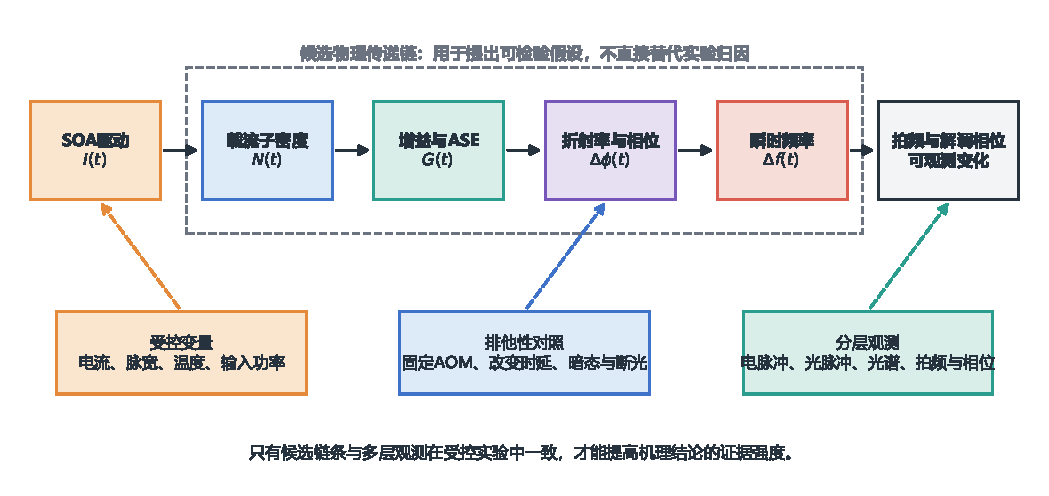
\includegraphics[width=0.96\textwidth]{images/chap2_soa_coupling_chain.pdf}
  \caption{SOA工作状态到外差拍频与解调相位的传递链路}
  \label{fig:chap2_soa_coupling_chain}
\end{figure}

\subsection{AOM移频与动态响应}

AOM利用射频信号在声光晶体中激发传播声波，形成移动折射率光栅。满足布拉格衍射条件时，一阶衍射光在改变传播方向的同时获得等于声波频率的光频移。若入射光频率为$f_0$，射频驱动频率为$f_A$，则一阶衍射光频率为

\begin{equation}
f_{\pm1}=f_0\pm f_A,
\label{eq:aom_shift}
\end{equation}

正负号由衍射级次和几何方向决定。将AOM置于信号支路或本振支路时，BPD接收的中频符号会改变，但实值采样频谱常表现为$|f_A|$附近的拍频\cite{pan2011phase,lu2010distributed}。

AOM射频开关并不会使衍射光功率瞬时改变。声波需要从换能器传播至光束区域，且声场前沿需要扫过有限光束宽度。若光束在声波传播方向上的有效直径为$d_b$，晶体声速为$v_a$，则响应时间量级为

\begin{equation}
\tau_A\sim\frac{d_b}{v_a}.
\label{eq:aom_rise}
\end{equation}

实际上升沿还取决于光束分布、换能器带宽、射频放大器和驱动波形\cite{johnson1977aom}。因此，SOA光脉冲若与AOM射频命令采用完全相同的开关边沿，光脉冲可能落在声场尚未稳定或正在消退的区域。已有φ-OTDR实验表明，AOM频率调制与脉冲斩波采用同源时钟可降低随机低频相位噪声\cite{yu2022lowfrequency_cn}；宽带声光多频调制和直接数字合成驱动则分别体现了频率分量控制与时序稳定的重要性\cite{lei2024broadband_cn,zhang2024highprecision}。

本文后续使用的时序关系可一般化表示为

\begin{equation}
t_{\mathrm{A,on}}
=
t_{\mathrm{SOA,on}}-\Delta t_{\mathrm{pre}},
\qquad
t_{\mathrm{A,off}}
=
t_{\mathrm{SOA,off}}+\Delta t_{\mathrm{hold}},
\label{eq:timing_compensation}
\end{equation}

其中，$\Delta t_{\mathrm{pre}}$和$\Delta t_{\mathrm{hold}}$分别为提前建立和延迟保持时间。式\eqref{eq:timing_compensation}只是时序设计变量定义，最佳参数应由光脉冲完整性、衍射效率、拍频稳定性、功耗和温升实验确定。

\section{外差相干探测与数字相位解调原理}

\subsection{外差拍频与平衡光电探测}

设瑞利回波信号光和本振光分别为

\begin{align}
E_s(t)&=\sqrt{P_s(t)}\exp\!\left[j(2\pi f_{\mathrm{sig}} t+\phi_s(t))\right],\\
E_{\mathrm{LO}}(t)&=\sqrt{P_{\mathrm{LO}}}\exp\!\left[j(2\pi f_{\mathrm{LO}}t+\phi_{\mathrm{LO}}(t))\right].
\end{align}

两路光由$2\times2$耦合器合束后进入理想BPD。两只光电二极管输出相减可抑制相同的直流光功率项，保留交叉拍频项。差分电流可写为

\begin{equation}
i_{\mathrm{BPD}}(t)
=
2R\sqrt{P_s(t)P_{\mathrm{LO}}}
\cos\!\left[
2\pi f_b t+\phi_s(t)-\phi_{\mathrm{LO}}(t)
\right]
+n_i(t),
\label{eq:bpd}
\end{equation}

其中，$R$为光电响应度，$f_b=|f_{\mathrm{sig}}-f_{\mathrm{LO}}|$为拍频，$n_i(t)$包含散粒噪声、热噪声、相对强度噪声和接收电子学噪声。平衡探测只在两臂增益、带宽和时延充分匹配时有效抑制共模分量；功率不平衡、BPD饱和和电缆差异都会降低共模抑制比\cite{lu2010distributed,pan2011phase,liokumovich2015fundamentals}。

若AOM仅位于其中一条支路，理想拍频主要由$f_A$确定。但激光频率漂移、SOA动态相位、AOM射频误差和采样时钟误差均可能使实际中频偏离标称值。因此，数字本振频率需结合实测频谱和时钟关系进行校核，而不能仅依据AOM标称频率设置。

\subsection{数字下变频与I/Q相位提取}

设采样后的实信号为

\begin{equation}
x[n]
=
A[n]\cos\!\left(2\pi f_b nT_s+\phi[n]\right)+w[n],
\label{eq:sampled_if}
\end{equation}

其中，$T_s=1/f_s$为采样间隔。数字下变频使用频率为$f_d$的正交本振：

\begin{align}
I_0[n]&=2x[n]\cos(2\pi f_d nT_s),\\
Q_0[n]&=-2x[n]\sin(2\pi f_d nT_s).
\end{align}

经低通滤波器$h[n]$去除和频项后，

\begin{align}
I[n]&=I_0[n]*h[n],\\
Q[n]&=Q_0[n]*h[n],
\end{align}

并构造复包络

\begin{equation}
S[n]=I[n]+jQ[n]=\hat A[n]\exp\!\left[j\hat\phi[n]\right].
\label{eq:complex_envelope}
\end{equation}

相位估计为

\begin{equation}
\hat\phi[n]
=
\operatorname{atan2}\!\left(Q[n],I[n]\right).
\label{eq:atan2}
\end{equation}

数字下变频、模拟I/Q、Sagnac平衡干涉和光学90度混合器是获得相位或复信号的不同实现形式，I/Q相位解调算法在不同实现条件下的适用性也得到系统比较\cite{fu2018iq,jiang2019analog,zhong2021sagnac,kong2025iq_thesis}。滤波器应覆盖有效拍频偏移和信号调制边带，同时抑制镜像、直流和带外噪声。中心频率错误、带宽过窄或过宽均可能损伤复包络\cite{zhang2025if,zhu2024downsampling}。

\subsection{频率失配、I/Q误差与差分解调}

当实际拍频$f_b$与数字本振$f_d$不一致时，低通后的复信号保留残余频率

\begin{equation}
\Delta f=f_b-f_d.
\label{eq:frequency_mismatch}
\end{equation}

此时

\begin{equation}
S[n]
\approx
\hat A[n]\exp\!\left\{
j\left[
2\pi\Delta f nT_s+\phi[n]
\right]
\right\},
\label{eq:residual_rotation}
\end{equation}

即I/Q矢量以$\Delta f$持续旋转。若处理窗内$2\pi\Delta f T$不可忽略，频率失配会表现为相位斜坡、滤波幅度变化或差分残差，并可能增加相位展开失败概率\cite{zhong2021frequency,qian2025drift}。

若I/Q通道存在幅度不平衡$\epsilon_g$、相位误差$\epsilon_\phi$、直流偏置和时延差$\Delta\tau$，观测复信号将由圆形轨迹变成偏移椭圆，并产生随频率变化的相位误差。另一方面，拍频漂移会在下变频后留下随时间累积的残余相位，近期研究已从频率漂移补偿角度改善φ-OTDR解调\cite{zhao2024frequency}。在双通道处理前应先进行直流去除、幅值归一、I/Q方向确认和时延校准。

本文对距离维信号采用式\eqref{eq:complex_difference}所示的复共轭差分，在相位求解前保持复数运算形式。低SNR区的相位概率分布会趋于发散，差分和相位展开无法恢复原本不存在的可靠信息\cite{lu2021detection,lu2022phaseerror,lu2023phase}；对距离--时间二维相位场，二维相位解卷绕方法可同时利用空间与时间方向的一致性抑制展开误差\cite{sun2024unwrapping_thesis}；大动态应变场景还需要处理相邻样点相位增量超过$\pi$时的解缠绕约束\cite{ran2025dynamic_thesis}。第4章将在实验参数表中给出空间步长、差分标距、滤波参数和有效区域，并在统一参数配置下评价系统性能。

\subsection{瑞利干涉衰落与低幅值相位失效}

式\eqref{eq:rayleigh_sum}中的多个随机散射相量可能在某些距离位置近似抵消，使合成复包络幅值$A=|S|$接近零。这种由相干瑞利散射随机叠加产生的局部深衰落称为瑞利干涉衰落或相干衰落。它不同于光纤平均损耗：平均损耗随距离缓慢变化，而干涉衰落表现为叠加在平均包络上的随机深谷，且衰落位置会随光频率、温度和应变状态变化\cite{tu2020fading,cheng2023subband,cui2021interference,lei2025fading_cn,shan2019key_thesis}。

将下变频后的I/Q噪声近似为方差相同且相互独立的高斯噪声，在高SNR小误差条件下，相位估计方差与复包络幅值平方近似成反比：

\begin{equation}
\operatorname{var}(\hat\phi)
\approx
\frac{\sigma_{IQ}^2}{A^2},
\label{eq:phase_variance_amplitude}
\end{equation}

其中，$\sigma_{IQ}^2$表示等效正交噪声方差。式\eqref{eq:phase_variance_amplitude}说明，当$A\rightarrow0$时，相位误差急剧增大；此时相位展开、空间差分或时间滤波都无法恢复原本缺乏可信度的信息。频率分集、脉冲编码、多频融合和选优合成可利用不同观测下衰落位置不完全重合的特点降低连续失效概率，但仍应设置幅值或功率可信度门限，避免对噪声主导的复数直接求相位。

\subsection{偏振衰落与双偏振接收}

单模光纤中的双折射随机变化使回波偏振态沿距离和时间演化。设信号光和本振光的归一化Jones矢量分别为$\mathbf e_s$和$\mathbf e_{\mathrm{LO}}$，相干拍频幅度与其内积模值成正比：

\begin{equation}
A_b
\propto
\left|
\mathbf e_{\mathrm{LO}}^{\mathrm H}\mathbf e_s
\right|.
\label{eq:polarization_inner}
\end{equation}

当两偏振近似正交时，$A_b$趋近于零，形成偏振衰落。PBS将回波分解到两个正交基，可得到$S_x$和$S_y$两个互补通道。理想情况下，总强度满足

\begin{equation}
P_{\Sigma}=|S_x|^2+|S_y|^2,
\label{eq:polarization_power}
\end{equation}

瑞利干涉衰落与偏振衰落的区别如图\ref{fig:chap2_fading_mechanisms}所示。前者来自同一分辨单元内随机散射相量的近似抵消，后者来自信号光与本振光Jones矢量投影过小；两者都表现为局部拍频幅值降低和相位噪声增加，但需要采用不同的缓解途径。

\begin{figure}[htbp]
  \centering
  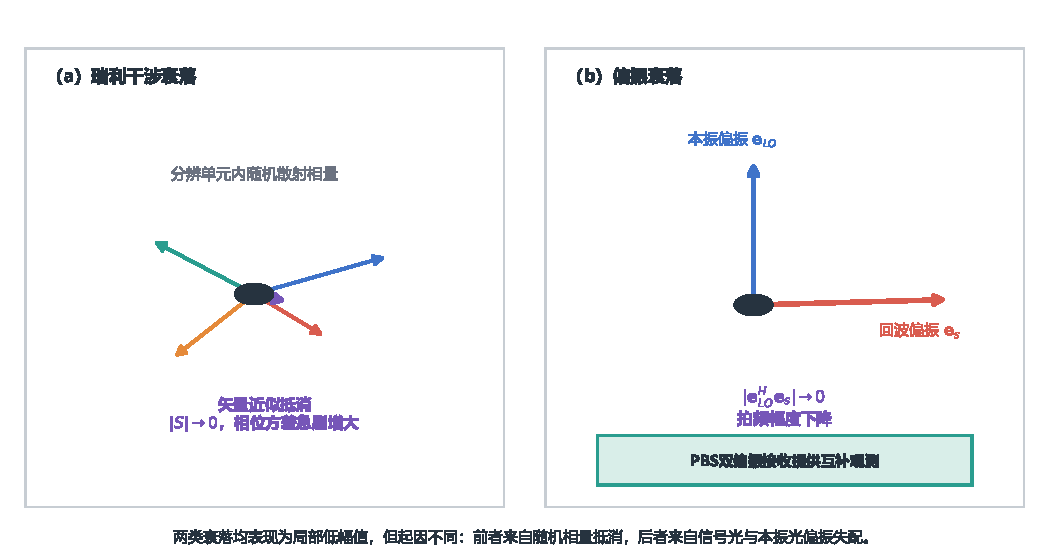
\includegraphics[width=0.96\textwidth]{images/chap2_fading_mechanisms.pdf}
  \caption{瑞利干涉衰落与外差相干接收中的偏振衰落机理}
  \label{fig:chap2_fading_mechanisms}
\end{figure}

但相位融合不能简单相加，因为两通道可能具有不同增益、直流偏置、I/Q方向、时延和固定相位。已有研究采用偏振分集接收、相干MIMO、偏振旋转和多维融合降低衰落\cite{dorize2018polarization,mompo2019distributed,tu2020fading,guerrier2020mimo,gorajoobi2022polarization,xie2023fading,sun2023polarization_thesis}。

本文采用功率加权双偏振合成。设校准后两通道复差分量为$C_x$和$C_y$，一种基于幅值可信度的合成形式为

\begin{equation}
C_{\mathrm{comb}}
=
w_x C_x+w_y C_y,
\qquad
w_x+w_y=1,
\label{eq:polarization_fusion}
\end{equation}

其中，权重可由通道幅值或信噪比确定。本文采用经通道标定后的功率加权形式进行双偏振合成，并将暗态及单臂断光噪声对照中总可信功率的99.9\%分位数设为门限；两路同时衰落时将对应位置标记为无效，不对噪声主导的复数求相位。具体规则在第4章与其他解调参数一并列出。

为使各公式在后续实验处理中具有清晰对应关系，图\ref{fig:chap2_fixed_demodulation_flow}汇总了本文采用的数字解调流程。P、S双偏振原始拍频完成偏置、幅值、I/Q方向和时延标定后，依次经过数字正交混频、低通滤波、复包络构造、复共轭空间差分、可信度判定和双偏振合成，最终获得用于定位、频率分析和波形恢复的差分相位。第4章将在统一参数配置下报告定位、频率和波形恢复结果。

\begin{figure}[htbp]
  \centering
  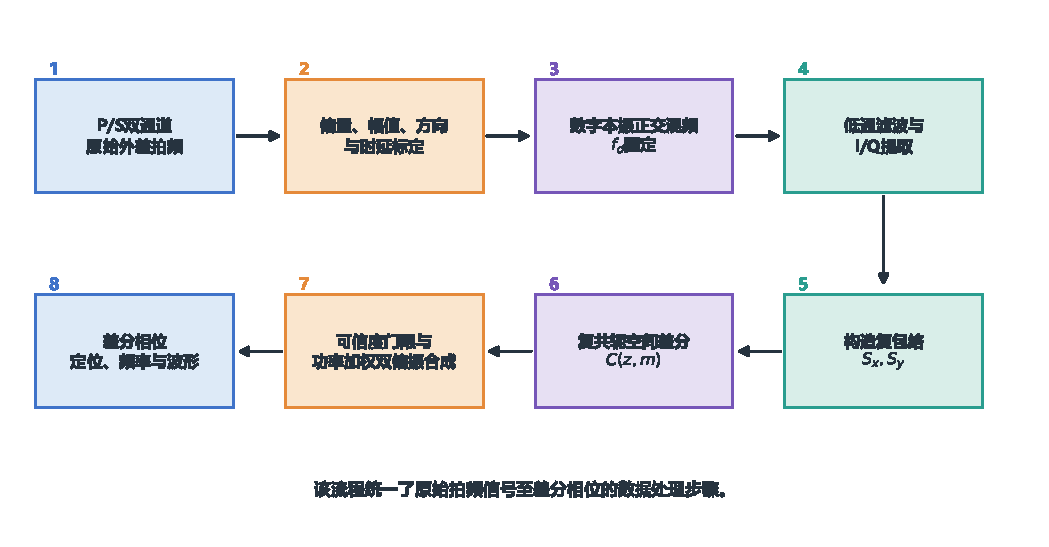
\includegraphics[width=0.96\textwidth]{images/chap2_fixed_demodulation_flow.pdf}
  \caption{数字下变频、复共轭差分与双偏振合成流程}
  \label{fig:chap2_fixed_demodulation_flow}
\end{figure}

\section{本章小结}

本章首先从传播相位全微分出发，说明声波引起的几何长度变化和光弹效应如何共同形成往返差分相位；随后建立相干瑞利后向散射的复场、概率统计、双程衰减和距离映射模型，对比传统OTDR、直接探测、自外差及外部本振相干探测方案，并系统说明空间分辨率、有效传感距离、应变分辨率、信噪比和响应带宽之间的约束关系。在此基础上，比较EDFA与SOA的增益介质、驱动方式、动态响应、噪声和集成特性，说明本文选择SOA是面向无EDFA紧凑发射链路的适配性取舍。

随后，本章利用载流子速率、增益传播和线宽增强因子说明集成SOA的ECL激光器中SOA的增益饱和、ASE及瞬态啁啾，利用声学渡越过程说明AOM移频和门控窗口，并推导外差BPD输出、数字下变频、I/Q相位提取、频率失配和复共轭差分模型。最后分别分析瑞利干涉衰落与偏振衰落，给出低幅值相位失效、双偏振接收和可信度门限的处理依据。

上述模型统一了后续实验的发射、移频、接收和解调变量。第三章据此完成一体化收发模组实验，第四章在统一参数下完成接收标定和数字相位解调验证。
